% Formato para un capítulo cualquiera

%Título del capítulo
\chapter{Introducción} 


Durante todo el siglo XX, en España, han ocurrido más de 7.000.000 de accidentes de tráfico \cite{sigloXX}, de los que en aproximadamente en 250.000 ha habido víctimas mortales \cite{vidas}. Un siglo después, gracias a la evolución de la tecnología, se crean los sistemas \ac{ISA}, que permiten establecer una velocidad aproximada para ayudar al conductor en cualquier situación de la vía.
%TODO: No me convence el párafo, pasas de los accidentes a los ISA dando un gran salto. Los sistemsa ISA no han aparecido un siglo después, por cierto, llevan tiempo. Modifica el párrafo para hilar ambas cosas. ¿Cuántos accidentes se deben a excesos de velocidad? ¿Hay cifras? Regular la velocidad es importante, existen lo sistemas ISA. Habla de soluciones comerciales (hay muchos modelos de coches que los llevan, basados en sistemas de detección de señales de tráfico, GPS y meta información, sensores de proximidad, etc).


Con la creación de estos sistemas se estima que el número de accidentes se reduciría considerablemente, y más importante aún, el número de víctimas \cite{reduccion}.


Sin embargo, estos sistemas, a pesar de tener buenas prestaciones, presentan algunos problemas. Esto es debido a que la mayoría de sistemas \ac{ISA} están basados en combinar la posición \ac{GPS} con meta-información asociada a la misma, en relación a la velocidad máxima permitida en la vía. Es decir, el módulo ISA comienza localizando mediante GPS la posición del vehículo, para luego consultar para esa posición, qué velocidad es la máxima permitida en dicha vía. Los principales problemas que pueden surgir, siguiendo este procedimiento, son los siguientes:
\begin{enumerate}
\item La información de la velocidad máxima de la vía puede que no esté actualizada, o que incluso sea incorrecta.
\item La precisión de la localización de los sistemas GPS en ocasiones puede resultar insuficiente para este tipo de sistemas. Por ejemplo, cuando circulamos por una vía de servicio paralela a una autovía, el sistema GPS puede no tener resolución suficiente para posicionarnos en el tipo de vía correcto. Nótese que los límites de velocidad son muy diferentes para estos dos tipos de vías (p. ej. 90 km/h versus 120 km/h), y el sistema ISA puede fallar.
\item No tienen en cuenta la situación real del tráfico, salvo si utilizan sensores de proximidad de otros vehículos, combinados con la información del GPS.
\end{enumerate}


Es por ello que aquí presentamos nuestro sistema capaz de resolver (en gran medida) estos problemas: \[ISA^{2}\]
%TODO: ¿Cómo? Anticipa en qué se basa: procesado de imagen.


\section{¿Qué es $ISA^{2}$? ¿Cómo funciona?}


La principal novedad de $ISA^{2}$ frente a los otros sistemas \ac{ISA} reside en la capacidad para analizar la situación real y actual del tráfico, y predecir, en consecuencia, la velocidad apropiada para ese instante. No se parte de información asociada a coordinadas GPS, sino que se emplean técnicas de inteligencia artificial y visión por computador para reconocer la situación de tráfico real, y poder recomendar una velocidad al conductor.


Para ello usamos una cámara en la parte frontal del vehículo que va tomando imágenes con una cierta frecuencia. Gracias a un sistema de \ac{SS}, conseguimos saber qué es cada cosa en cada foto, es decir; qué píxeles son los correspondientes a un vehículo, peatón, semáforo, acera, etc. Con esa información se construye un vector de características que será empleado por los módulos de inteligencia artificial para realizar una regresión o estimación de la velocidad a la que se debe circular.

%TODO: mejor que una imagen con solo datos de segmentación semántica, debes incluir una imagen donde se vea todo, desde la imagen original, a la segmentación semántica, y al proceso de extracción de características y la regresión final. Es para dar una idea gráfica del problema. Una vez la tengas, la metes y la comentas en el propio texto. Te dejo lo de abajo comentado para que lo cambies.
%He aquí un ejemplo de una imagen real \ref{fig:ImgOrig} y de la misma imagen procesada por el sistema de \ac{SS} \ref{fig:ImgSegm}:

%\begin{figure}[h]
%  \centering
%  \includegraphics[width=12cm]{Figuras/Imagen_Original.eps}
%  \caption{Imagen Original}
%  \label{fig:ImgOrig}
%\end{figure}

%\begin{figure}[h]
%  \centering
%  \includegraphics[width=12cm]{Figuras/Ejemplo_Imagen_Segmentada.eps}
%  \caption{Imagen Segmentada}
%    \label{fig:ImgSegm}
%\end{figure}


\section{Objetivo principal}


El objetivo principal de este proyecto es la optimización del sistema $ISA^{2}$ y para ello lo que hemos hecho ha sido un largo proceso de análisis de sistemas de \ac{SS}, acompañado de la dificultad que éstos conllevan para poder ejecutarlos correctamente. Tras ello, hemos recogido los datos generados por dicho sistema, los hemos evaluado para obtener las velocidades correspondientes, y hemos comparado éstas con las de la primera versión de $ISA^{2}$, obteniendo resultados muy prometedores.


En la primera versión se utilizó un framework llamado \textbf{DeepLab} \cite{deeplab} para realizar el proceso de segmentación semántica con unos resultados muy buenos. Para este proyecto, a través de una exhaustiva búsqueda de modelos y tras muchas pruebas, hemos utilizado uno conocido como \textbf{Swiftnet} \cite{swiftnet}, el cual conlleva una mejora realmente interesante.

Afortunadamente, Swiftnet es un modelo de código abierto en GitHub de modo que cualquiera puede utilizarlo a su disposición \cite{github_swiftnet}. Todo lo que hay que hacer es clonar el repositorio en el que se encuentra utilizando el siguiente comando en la terminal del sistema \cite{clonar}:

\begin{center}
\textit{git clone URL\_del\_repositorio}
\end{center}

Cuando clonemos el repositorio, se recomienda hacerlo desde el escritorio (carpeta \textbf{Desktop}) para ejecutar Swiftnet según este trabajo.

En el siguiente capítulo, explicaremos en detalle el proceso que realiza $ISA^{2}$ parte por parte, y los pasos que hemos seguido para conseguir que todo funcione correctamente.

\section{Campos de aplicación}


Este proyecto será aplicable a cualquier campo relacionado con el automovilismo, para ayudar a mejorar la seguridad vial actual y para facilitar la lectura de la vía durante la conducción. A modo de resumen, podríamos plasmar las ideas recogidas de todo lo anterior en los siguientes puntos:
\begin{enumerate}	
	\item Implementación de soluciones de adaptación de velocidad inteligente.
	\item Implementación de sistema de detección de situaciones peligrosas en función de la velocidad.
	\item Desarrollo de nuevas ayudas a la conducción más inteligentes.
\end{enumerate}

\section{Medios disponibles}

Dispondremos de las siguientes herramientas:

\begin{enumerate}
	\item Estación de trabajo con \textbf{GPU (NVIDIA 1080 TI)} para la realización de experimentos con sistema operativo \textbf{Ubuntu}.
	\item Acceso a la librería de \textbf{Deep Learning} llamada \textbf{PyTorch} \cite{pytorch}
	\item Acceso a la base de datos $ISA^2$ utilizada en la primera versión \cite{isa2} a través del siguiente enlace: \url{http://agamenon.tsc.uah.es/Personales/rlopez/data/isa2/index.html}.
\end{enumerate}
%\section{¿Cómo escribir tu PFC en \LaTeX{} ?}

%Escribir un \ac{PFC} es una tarea de gran importancia. La herramienta de edición \LaTeX{} te va a permitir editar tu \ac{PFC} de una forma elegante, útil y segura. Simplemente dedicando unos minutos a comprender cómo están organizados los ficheros que acabas de descargar, y realizando algunas pruebas con ellos, podrás comenzar a escribir el tuyo.

%\subsection{La mejor manera para aprender a programar es programando}

%\LaTeX{} es un lenguaje de programación como tantos otros a los que estás acostumbrado. Puedes encontrar mucha información y manuales en Internet, siendo el mejor sitio \cite{LatexWiki}. También te recomiendo las referencias siguientes: \cite{Latex1} y \cite{Latex2}.

%Este documento PDF que estás leyendo ha sido generado mediante \LaTeX{} utilizando los ficheros:
%\begin{enumerate}
%\item \textit{tfc.tex} : es el fichero principal, desde él se hacen las llamadas a los demás ficheros, que pueden ser editados de forma independiente. Si abres este fichero con cualquier editor de textos verás que contiene muchas sentencias que ahora desconoces. Puedes observar que el fichero tiene una zona de cabecera donde se incluyen todos los paquetes a utilizar. Luego se define el título del documento y su autor, para, al final, ir añadiendo los capítulos y secciones de tu \ac{PFC}.
%\item \textit{previo.tex}: genera la hoja de calificación oficial para un \ac{PFC} de la Universidad de Alcalá.
%\item \textit{dedicatoria.tex}: para que escribas tus dedicatorias.
%\item \textit{agradecimientos.tex}: para que escribas los agradecimientos, que seguro son muchos.
%\item \textit{resumen.tex}: aquí debes escribir un resumen de tu trabajo.
%\item \textit{introduccion.tex}: este es un capítulo modelo, en el que encontrarás los comandos utilizados para generar lo que estás ahora mismo leyendo.
%\item \textit{apendice-a.tex}: un modelo de apéndice, muy utilizado en un \ac{PFC} cuando queremos incluir en el documento final código fuente, manuales de usuario, \ldots
%\item \textit{bibliografia-pfc.bib} : este es un fichero \textit{.bib} (no lleva la extensión .tex como los anteriores). Es un fichero de bibliografía \textbf{BibTex}. La bibliografía es una parte fundamental de un \ac{PFC}, y es por ello que debemos poner especial cuidado a la hora de editarla, ya que va a permitir que futuros lectores de tu \ac{PFC}, que seguro serán muchos, puedan acudir a las referencias cuando no entiendan algo, o cuando pretendan retomar tu trabajo y continuar con él para mejorarlo. Sobre BibTex también existen muchos manuales, pero encontrarás información útil en \cite{bibtex1}. Para manejar tu bibliografía te recomiendo el programa JabRef\footnote{En Ubuntu está disponible, o si prefieres, puedes descargar la última versión de la página oficial \url{http://jabref.sourceforge.net/}}.
%\end{enumerate}

%Para probar que todo esto funciona sólo tienes que compilar el fichero \textit{tfc.tex}, ¿pero cómo?. %Evidentemente necesitas un compilador. Veamos que opciones existen:

%\begin{enumerate}
%\item \textbf{\underline{Plataforma Linux (Unix)}}: simplemente necesitas tener instalado el compilador \textit{latex}, que suele estar incluido en un paquete con el mismo nombre. Existe un entorno de trabajo bastante agradable y útil, que es \textit{Kile}, sobre el que podrás editar tus documentos de forma cómoda, gráfica y sencilla. También puedes utilizar la herramienta \textit{Lyx}, que te permite saber cómo va quedando tu documento a medida que escribes, sin necesidad de primero editar el código y luego compilar, es decir, es un software de filosofía WYSIWYM (What You See Is What You Mean).
%\item \textbf{\underline{Otras plataformas}}: para trabajar con \LaTeX{} sobre otros sistemas operativos dispones de gran cantidad de software. Simplemente voy a indicarte algunas herramientas que son de libre distribución:
%\begin{itemize}
%\item Compilador: el único que conozco es \textit{MikTex}, lo puedes descargar de su web oficial.
%\item Editor: puedes utilizar TeXnicCenter o WinShell, ambos de libre distribución.
%\end{itemize}
%\end{enumerate}

%Una sugerencia: \textbf{\textit{¿no crees que es un buen momento para trabajar desde Linux?}}. Si no tienes este sistema operativo en tu ordenador, prueba a instalar la distribución \textit{Ubuntu} (http://www.ubuntu.com), es realmente sencillo funcionar con ella, y además puedes descargarla desde la web o incluso pedir un cd de forma totalmente gratuita.


%Ahora que conoces algunas herramientas, debes probar a compilar el fichero \textit{tfc.tex} hasta que obtengas como resultado este pdf.

%\subsection{Algunos detalles más}

%Con \LaTeX{} puedes editar tus propias tablas (Tabla \ref{tabla:primera}), e incluso añadir gráficos a tus documentos (Figura \ref{grafico:primero}). A la hora de añadir un gráfico la mejor opción es trabajar con formatos de imagen \textit{.eps}, vectorial preferiblemente, aunque puedes incrustar imágenes en formato bmp, jpg y otros muchos.

%\begin{table}
%\begin{center}
%\begin{tabular}{|c|c|c|}\hline
%\textbf{Medida} & \textbf{Error} & \textbf{Porcentaje} \% \\ \hline
%12 & 23.6 & 22 \\ \hline
%-1 & 13 & 4 \\ \hline
%6 & 3 & 4 \\ \hline
%\end{tabular}
%\caption[El título corto de la tabla.]{El título de la tabla.}
%\label{tabla:primera}
%\end{center}
%\end{table}

%\begin{figure}
%\begin{center}
%Para compilar con latex
%
\includegraphics[width=4cm]{Figuras/LogoUAH.eps}\\
%Para compilar con pdflatex
%
\includegraphics[width=4cm]{Figuras/LogoUAH.png}\\
%\end{center}
%\caption[El título corto de la gráfica.]{El título de la gráfica.}
%\label{grafico:primero}
%\end{figure}


%\LaTeX{} también te permite editar ecuaciones de forma muy sencilla y realmente elegante, observa.
%\begin{equation}
%I = \! \int_{-\infty}^\infty f(x)\,dx \label{eq:fine}.
%\end{equation}

%\begin{equation}
%\label{eq:mdiv}
%m(T) =
%\begin{cases}
%0 & \text{$T > T_c$} \\
%\bigl(1 - [\sinh 2 \beta J]^{-4} \bigr)^{\! 1/8} & \text{$T < T_c$}
%\end{cases}
%\end{equation}

%\begin{align}
%\textbf{T} &=
%\begin{pmatrix}
%T_{++} \hfill & T_{+-} \\
%T_{-+} & T_{--} \hfill 
%\end{pmatrix} , \nonumber \\
%& =
%\begin{pmatrix}
%e^{\beta (J + B)} \hfill & e^{-\beta J} \hfill \\
%e^{-\beta J} \hfill & e^{\beta (J - B)} \hfill
%\end{pmatrix}.
%\end{align}

%\section{Recomendaciones importantes}
%Antes de enviarme un copia de tu trabajo para revisar, asegúrate de que has realizado las siguientes tareas:
%\begin{enumerate}
 %\item Pasar un corrector ortográfico. Kile trae uno incorporado. No seguiré revisando ningún documento que contenga más de 3 faltas de ortografía.
 %\item Leer lo que hemos escrito y revisarlo hasta que tenga coherencia. No seguiré revisando ningún documeto que contenga más de 3 frases que no se entiendan.
 %\item Todas la figuras que se incluyen deben citarse en el texto. Lo mismo ocurre con las tablas. Debes aprender a manejar los comandos \verb+\label+ y \verb+\ref+.
 %\item La Bibliografía es FUNDAMENTAL. Cita bien y cita mucho.  Debes aprender a manejar el comando \verb+\cite+ y a tener una base de datos con todas tus lecturas en formato BibTex.
 %\item En la redacción del proyecto procura mantener un estilo serio. Se trata de un documento oficial.
%\end{enumerate}


%\section{Para terminar}
%En el fichero \textit{introduccion.tex} encontrarás todo el código que se ha utilizado para generar este capítulo, échale un vistazo y trata de entender todo aquello que está escrito en él. Si consigues generar este documento pdf de nuevo, es que estás preparado para editar tu propio \ac{PFC} incluyendo los nuevos capítulos que necesites.

%\begin{center}
%\begin{large}\textbf{Adelante y buena suerte.}\end{large}
%\end{center}

